% FREUID Challenge 2026 — Technical Report
% Compile: pdflatex technical_report.tex && bibtex technical_report && pdflatex x2

\documentclass[11pt,a4paper]{article}

\usepackage[T1]{fontenc}
\usepackage[utf8]{inputenc}
\usepackage{lmodern}
\usepackage{microtype}
\usepackage{geometry}
\usepackage{graphicx}
\usepackage{booktabs}
\usepackage{amsmath}
\usepackage{hyperref}
\usepackage{xcolor}
\usepackage{enumitem}
\usepackage{subcaption}
\usepackage{float}

\geometry{margin=2.5cm}
\hypersetup{
  colorlinks=true,
  linkcolor=blue!60!black,
  citecolor=blue!60!black,
  urlcolor=blue!60!black,
}

\newcommand{\teamname}{akhil838}
\newcommand{\kaggleteam}{akhil838}
\newcommand{\contactemail}{kosuriakhil19@gmail.com}
\newcommand{\reportdate}{\today}

\title{%
  \textbf{The FREUID Challenge 2026}\\[0.4em]
  \large Technical Report --- \teamname
}
\author{%
  Akhil Kosuri\\
  \small Independent researcher\\
  \texttt{\contactemail}
}
\date{Report date: \reportdate}

\begin{document}
\maketitle
\sloppy

\begin{abstract}
We present a two-branch forensic pipeline for identity document fraud detection
that separately targets photo manipulation and text-field tampering.
For photo fraud, we train a unified DINOv2-small classifier (22M parameters) on
MediaPipe BlazeFace-detected portrait crops across all five document types, achieving 99.4\%
validation accuracy.
For text fraud, we decompose each document into per-field forensic panels ---
$224 \times 1008$ six-view composites capturing grayscale, ink mask, luminance
residual, chroma residual, texture variance, and edge magnitude --- and train
a ConvNeXt-Base classifier (88M parameters) on 65{,}413 panels combining real
annotated tampered fields, synthetic-on-real augmentations (9 effect types), and
fully synthetic rendered fields.
Document-level fraud scores are computed as $\max(\text{photo\_prob}, \text{text\_prob})$,
where text probability uses max-field aggregation.
On the FREUID public leaderboard, our solution achieves a score of \textbf{0.294}
(lower is better). Training was performed on an Apple M3~Max;
inference runs in approximately 2.7 hours on an NVIDIA A100 for 142{,}818 documents.
All code, weights, and annotations are released for full reproducibility.
\end{abstract}

\noindent\textbf{Competition:} The FREUID Challenge 2026 (IJCAI-ECAI 2026)\\
\textbf{Kaggle team:} \kaggleteam\\
\textbf{Code:} \url{https://github.com/akhil838/doc-forensic-pipeline}\\
\hspace*{1.5cm}(commit \texttt{0d51c75d})\\
\textbf{Weights:} \url{https://huggingface.co/akhil838/doc-forensic-models-v1}\\
% ============================================================================
\section{Introduction}
\label{sec:intro}

The FREUID Challenge~\cite{freuid2026} targets next-generation identity document
fraud spanning physical manipulations, GenAI-driven digital edits, and
print-and-capture attacks across five country/document types
(Benin/DL, Egypt/DL, Guinea/DL, Mauritius/ID, Mozambique/DL).

Our key insight is that document fraud decomposes into two independent subtasks
--- \emph{photo/face tampering} and \emph{text-field tampering} --- and each is
best addressed with a specialized detection branch.
For photo fraud, the face region carries the signal; for text fraud, local
forensic inconsistencies within individual text fields (ink density, background
residuals, edge halos) are more discriminative than global image features.

% ============================================================================
\section{Method}
\label{sec:method}

\subsection{Pipeline overview}

Our inference pipeline processes each document image through five stages
(Figure~\ref{fig:pipeline}):

\begin{enumerate}[noitemsep]
  \item \textbf{Face detection} --- MediaPipe BlazeFace localizes the portrait
        photo (2\,ms/image, CPU).
  \item \textbf{Face classification} --- The detected face region is expanded to
        a standardized portrait crop ($256 \times 320$), resized to
        $224 \times 224$, and classified by a DINOv2-small model
        (1.2\,ms/face, GPU).
  \item \textbf{Text field detection} --- PaddleOCR PP-OCRv6~\cite{paddleocr} detects all text
        field bounding boxes (35\,ms/image, GPU).
  \item \textbf{Forensic panel scoring} --- Each filtered text field is cropped
        with context padding, converted to a $224 \times 1008$ six-view forensic
        panel, and scored by a ConvNeXt-Base classifier
        (1.5\,ms/field, GPU).
  \item \textbf{Score aggregation} --- Document fraud score is
        $\max(\text{photo\_prob},\; \max_i(\text{field\_prob}_i))$.
\end{enumerate}

\begin{figure}[H]
  \centering
  % PLACEHOLDER: replace with pipeline diagram
  
\includegraphics[width=\textwidth]{figures/prediction_pipeline.png}
  \caption{End-to-end inference pipeline. Two branches operate independently and
           their scores are combined via max.}
  \label{fig:pipeline}
\end{figure}

\subsection{Face detection and classification}

We use MediaPipe BlazeFace~\cite{blazeface,mediapipe} for face detection, selecting the largest left-side
face (primary portrait region). The detected face square is expanded by a factor
of $2.15\times$ to capture the full portrait area, then regularized to a stable
document-height fraction ($42$--$72\%$) with fixed $256{:}320$ aspect ratio.
When no face is detected, a generic left-side portrait fallback crop is used.

The portrait crop is classified by a DINOv2-small backbone~\cite{dinov2}
(\texttt{facebook/dinov2-small}, 22M parameters) with a
LayerNorm$(384)$ $\rightarrow$ Dropout$(0.1)$ $\rightarrow$ Linear$(384, 2)$ head.
All backbone parameters are trainable with differential learning rates
(backbone: $10^{-5}$, head: $3 \times 10^{-4}$).
The model is trained on balanced samples (20{,}440 per class) across all five
countries, achieving \textbf{99.4\% accuracy} and \textbf{AUC\,=\,0.9998} on
validation.

\begin{figure}[H]
  \centering
  % PLACEHOLDER: face detection + crop examples
  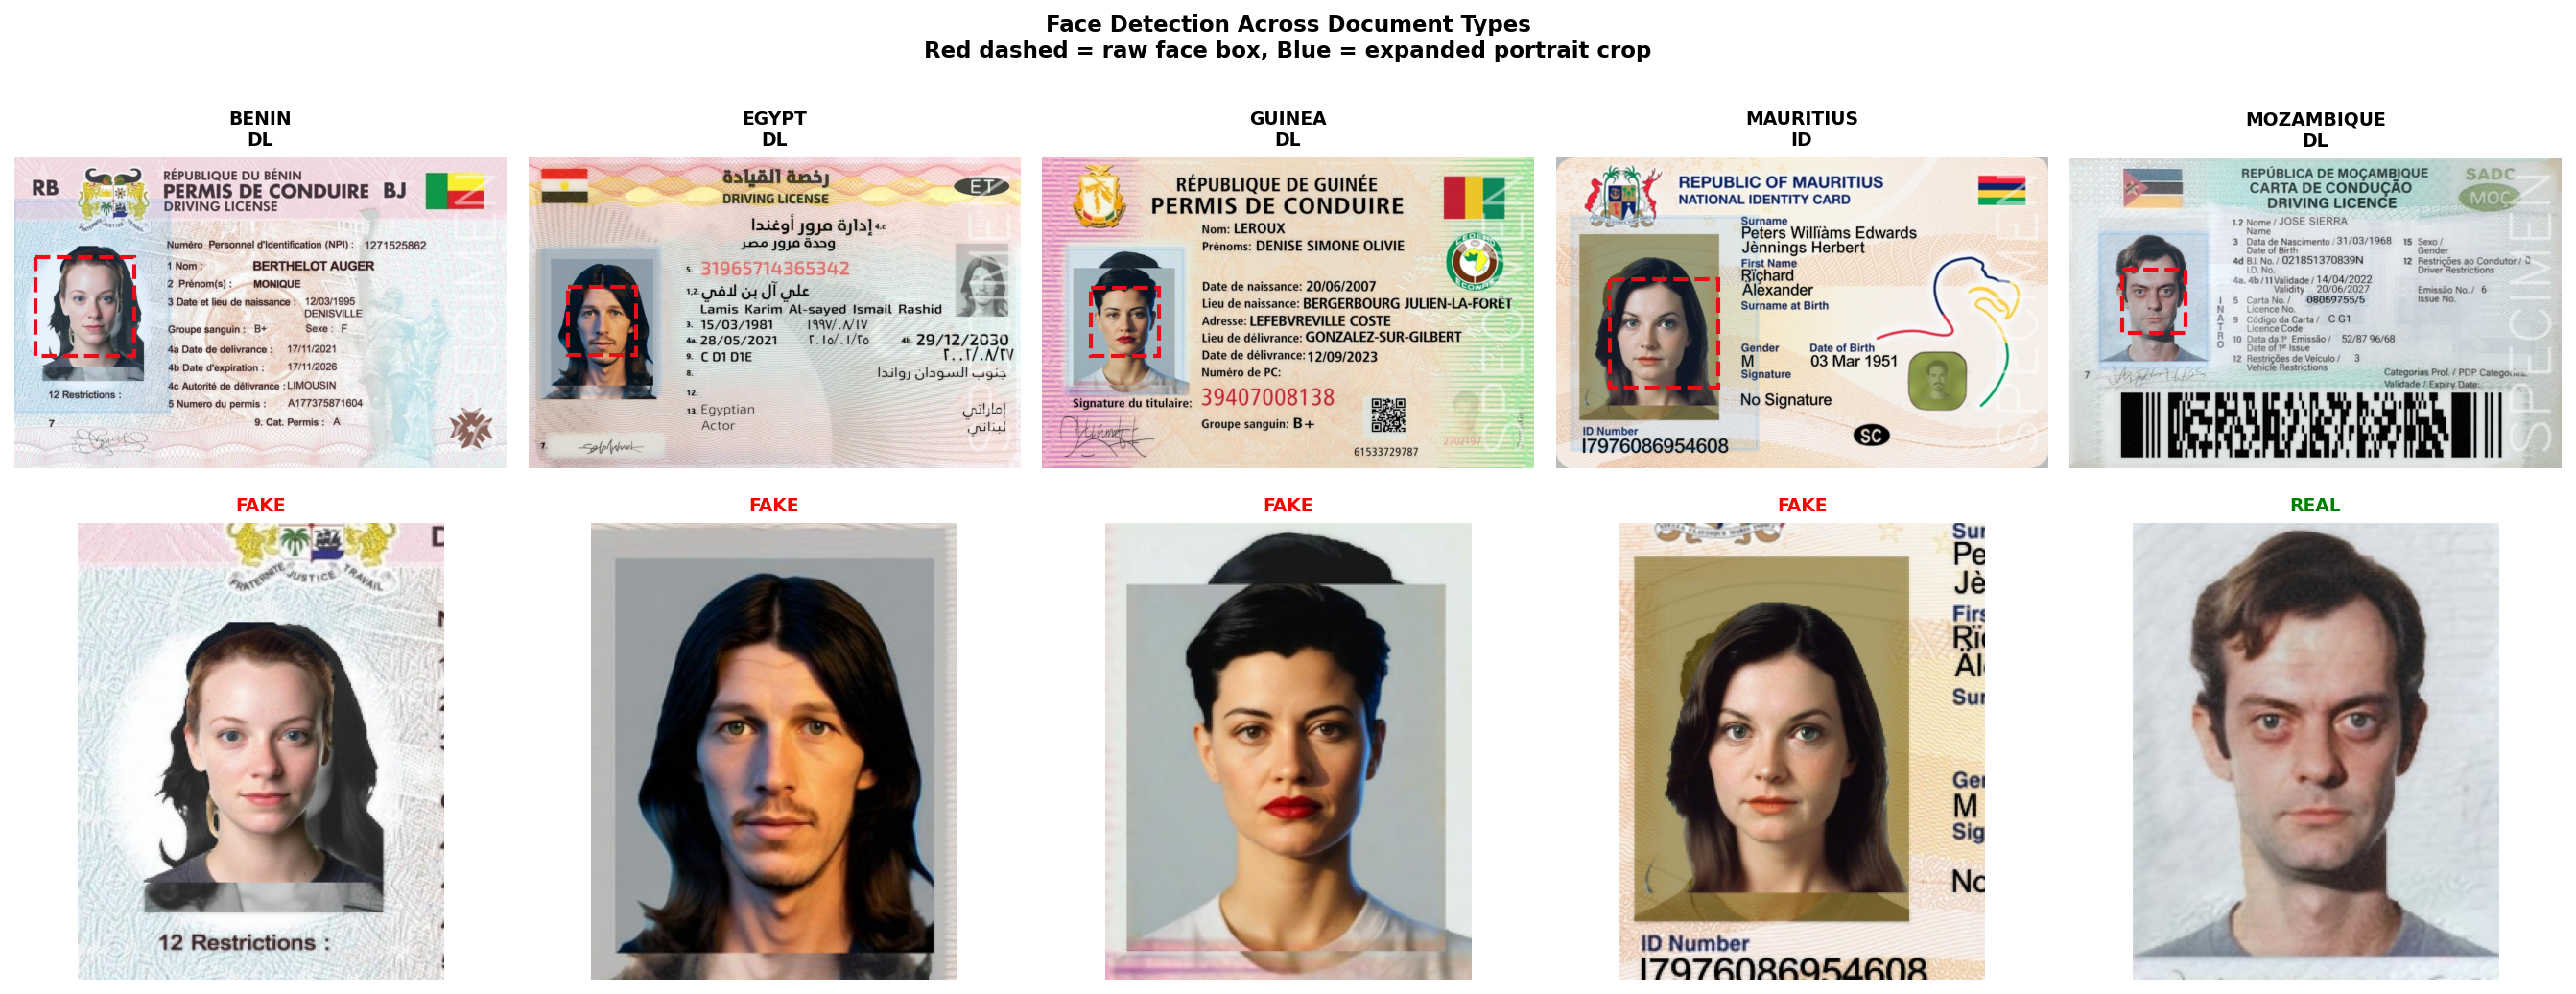
\includegraphics[width=\textwidth]{figures/face_detection_examples.png}
  \caption{Face detection and portrait crop extraction across document types.}
  \label{fig:face_examples}
\end{figure}

\subsection{Text field detection and filtering}

PaddleOCR PP-OCRv6 (medium detection model, 62\,MB) detects all text-like regions
in each document. Raw detections are filtered to remove non-text elements:

\begin{table}[H]
  \centering
  \small
  \caption{Text field filtering parameters (identical at training and inference).}
  \label{tab:filtering}
  \begin{tabular}{llp{7cm}}
    \toprule
    Filter & Threshold & Rationale \\
    \midrule
    Header band    & $y_0 < 0.17 \cdot H$  & Skip document title, flag, header region \\
    Minimum size   & $w < 10$ or $h < 8$    & Remove noise dots, decoration fragments \\
    Aspect ratio   & $w/h < 0.5$            & Remove vertical borders, decorative lines \\
    Maximum height & $h > 0.09 \cdot H$     & Remove flags, photos, QR codes \\
    Maximum width  & $w > 0.85 \cdot W$     & Remove full-width header bars \\
    Field cap      & 40 per document        & Limit computation \\
    \bottomrule
  \end{tabular}
\end{table}

After filtering, each field is cropped with $15$\,px horizontal and $5$\,px
vertical context padding.

\subsection{Forensic panel generation}

Each text field crop is converted to a $224 \times 1008$ six-view forensic panel
(Figure~\ref{fig:forensic_panel}). The crop is first letterboxed to
$112 \times 336$ (fill value 245, matching typical document background), then
processed into six grayscale views arranged in a $2 \times 3$ grid:

\begin{enumerate}[noitemsep]
  \item \textbf{Grayscale} --- raw luminance; reveals font weight and style
        inconsistencies.
  \item \textbf{Ink mask} --- adaptive thresholding
        ($\text{gray} < \text{local\_mean} - 22$ and $< 175$, or $< 80$) with
        $3 \times 3$ dilation; detects reprinted text with different ink coverage.
  \item \textbf{$|L|$ residual} --- CIELAB luminance after Gaussian
        background subtraction ($\sigma = \max(8, \min(W,H)/8)$); reveals
        inserted or pasted content against the original background.
  \item \textbf{Chroma residual} --- $\sqrt{A'^2 + B'^2}$ after background
        subtraction; detects color inconsistency from different paper or ink.
  \item \textbf{Texture variance} --- local standard deviation ($15 \times 15$
        window); smooth reprinted patches contrast with textured originals.
  \item \textbf{Edge magnitude} --- Sobel gradient; reveals halos, blurring, or
        sharpening artifacts at tamper boundaries.
\end{enumerate}

\begin{figure}[H]
  \centering
  % PLACEHOLDER: forensic panel examples
  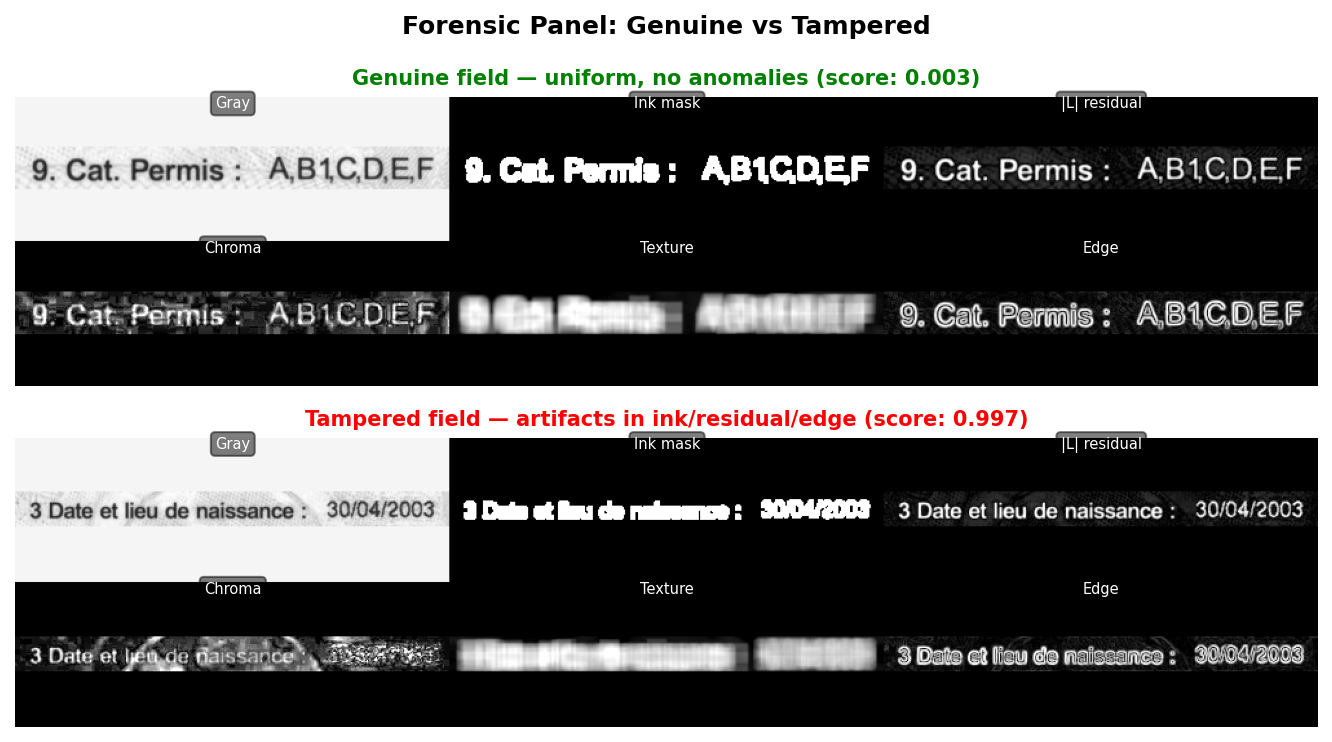
\includegraphics[width=\textwidth]{figures/forensic_panel_example.png}
  \caption{Six-view forensic panels. Top row: grayscale, ink mask, $|L|$ residual.
           Bottom row: chroma residual, texture variance, edge magnitude.
           Tampered fields show visible anomalies in residual and edge views.}
  \label{fig:forensic_panel}
\end{figure}

\subsection{Text tamper classifier (ConvNeXt-Base)}

The forensic panels are classified by a ConvNeXt-Base backbone~\cite{convnextv2} initialized from
{\small\texttt{facebook/dinov3-convnext-base-pretrain-lvd1689m}} (88M parameters).
The last 2 ConvNeXt stages and the layer normalization are unfrozen during
fine-tuning; earlier stages remain frozen.
The classification head is:
Linear$(1024, 256)$ $\to$ GELU $\to$ Dropout$(0.15)$ $\to$ Linear$(256, 1)$.

\subsubsection{Training data composition}

Training panels are assembled from three sources (Table~\ref{tab:panels}):

\begin{table}[H]
  \centering
  \small
  \caption{Training panel composition (65{,}413 total, positive fraction 38.9\%).}
  \label{tab:panels}
  \begin{tabular}{llrr}
    \toprule
    Source & Label & Count & Description \\
    \midrule
    Real tampered fields       & 1 & 5{,}001 & From 6{,}764 annotated documents \\
    Genuine negatives          & 0 & 36{,}000 & Clean fields from tampered + clean docs \\
    Synth-on-real (9 effects)  & 1 & 16{,}000 & Tamper effects applied to real clean crops \\
    Fully synthetic clean      & 0 & 4{,}000  & Rendered text, no tampering \\
    Fully synthetic tampered   & 1 & 4{,}000  & Rendered text + tamper effect \\
    \midrule
    \textbf{Total}             &   & \textbf{65{,}413} & pos\_frac = 0.389 \\
    \bottomrule
  \end{tabular}
\end{table}

\subsubsection{Synthetic tamper effects}

Nine ink-aware tamper effects simulate real-world document manipulation
(Figure~\ref{fig:synth_effects}):

\begin{enumerate}[noitemsep]
  \item \texttt{smooth\_row\_shift} --- per-row horizontal displacement of ink
        pixels (mimics captured row-shift tampering).
  \item \texttt{copy\_move} --- duplicate a character span at a shifted location.
  \item \texttt{clean\_text\_reprint} --- erase original ink, re-render with a
        new font/text (Guinea-style patch-and-rewrite).
  \item \texttt{cool\_blue\_bg\_filter} --- cool/blue color filter on the
        background within the text bounding box.
  \item \texttt{bg\_color\_morph} --- shift/boost background pixel colors while
        preserving text and pattern structure.
  \item \texttt{diffusion\_spread} --- MNIST-style stroke irregularity with
        smooth alpha-blended segment dilation.
  \item \texttt{non\_ink\_background\_noise} --- Gaussian noise + shifted-copy
        exchange on background pixels.
  \item \texttt{faint\_horizontal\_lines} --- colored horizontal lines through
        text rows.
  \item \texttt{field\_static\_noise} --- TV-static speckle noise.
\end{enumerate}

All effects operate on ink-masked regions using the same adaptive ink detection
as the forensic panel builder.
Synthetic-on-real effects are applied to genuine clean field crops; fully
synthetic effects are applied to rendered text on diverse mathematical
background patterns.
A capture degradation step (exposure jitter, resolution loss, optical blur,
sensor noise, JPEG recompression) is applied to all synthetic panels.

\begin{figure}[H]
  \centering
  % PLACEHOLDER: synthetic effect examples
  
\includegraphics[width=\textwidth]{figures/synth_effects_grid.png}
  \caption{Nine synthetic tamper effects used for training data augmentation.}
  \label{fig:synth_effects}
\end{figure}

\subsection{Training objective and procedure}

\begin{itemize}[noitemsep]
  \item \textbf{Loss:} BCEWithLogitsLoss with $\text{pos\_weight} = 1.5$
        (mild upweighting of tampered panels to compensate for 38.9\% positive
        fraction).
  \item \textbf{Optimizer:} AdamW, $\text{lr} = 2 \times 10^{-5}$,
        $\text{weight\_decay} = 0.01$.
  \item \textbf{Schedule:} Cosine annealing over all training steps.
  \item \textbf{Gradient clipping:} max norm 1.0.
  \item \textbf{Epochs:} 6, best checkpoint selected at epoch~2 by validation
        document-level AUC on 1{,}807 held-out training documents
        (1{,}314 text-fake, 493 clean).
  \item \textbf{Batch size:} 12.
  \item \textbf{Seed:} 42 for all random operations.
\end{itemize}

\subsubsection{Data augmentations (applied at training time)}

\begin{itemize}[noitemsep]
  \item HSV hue shift ($\pm 30$, 60\%) and saturation jitter ($0.7$--$1.3\times$).
        \emph{Note:} forensic panels are grayscale, so this augmentation has no
        effect in practice --- a known limitation.
  \item Brightness/contrast jitter ($\alpha \in [0.7, 1.3]$, $\beta \in [-20, 20]$, 50\%).
  \item Gaussian blur ($k \in \{3, 5\}$, 20\%).
  \item JPEG recompression ($Q \in [30, 80]$, 30\%).
  \item Gaussian noise ($\sigma \in [3, 12]$, 20\%).
  \item Horizontal flip (50\%), vertical flip (20\%).
\end{itemize}

\subsection{Score aggregation and calibration}

Per-field logits are passed through sigmoid to obtain probabilities in $[0, 1]$.
The document-level text score is the \textbf{maximum} field probability:
\[
  \text{text\_prob} = \max_{i=1}^{N} \sigma(\text{logit}_i)
\]
where $N$ is the number of filtered fields (typically 15--25 per document).
We chose max aggregation over top-$k$ mean because tampering typically affects
only 1--2 fields; averaging dilutes the signal.

The final fraud score combines both branches:
\[
  \text{fraud\_score} = \max(\text{photo\_prob},\; \text{text\_prob})
\]

No additional calibration, temperature scaling, or post-processing is applied.

% ============================================================================
\section{Data}
\label{sec:data}

\subsection{FREUID training set}

We used all 69{,}352 official training images.
Document-level labels were decomposed into subtask annotations
(\texttt{photo\_cutout} vs \texttt{details\_tamper}) using a combination of
model predictions and manual verification.
For the 2{,}137 Mozambique/DL fraud images that were initially unclassified,
we used the trained face model to auto-assign photo vs text labels (bimodal
confidence distribution: all predictions $>0.95$ or $<0.05$).

Field-level annotations were created using a custom browser-based annotation
tool (\texttt{field\_annotation\_server.py}) that overlays PaddleOCR field
boxes on document images. Annotators clicked specific tampered fields,
producing per-field indices and pixel coordinates.
A total of 6{,}764 training documents received field-level annotations.

\subsection{External data and pre-trained models}

\begin{table}[H]
  \centering
  \small
  \caption{External resources used.}
  \begin{tabular}{lll}
    \toprule
    Resource & License & Usage \\
    \midrule
    \texttt{facebook/dinov3-convnext-base-pretrain-lvd1689m} & Apache 2.0 & Text classifier backbone \\
    \texttt{facebook/dinov2-small} & Apache 2.0 & Face classifier backbone \\
    PaddleOCR PP-OCRv6 medium det & Apache 2.0 & Text field detection \\
    MediaPipe BlazeFace & Apache 2.0 & Face detection \\
    \bottomrule
  \end{tabular}
\end{table}

No external training data was used beyond the FREUID competition dataset and
publicly licensed pre-trained model weights.

\subsection{Validation strategy}

For the text model, validation is performed on 1{,}807 held-out training
documents (sampled from \texttt{subtask\_annotations.csv}: 1{,}314 text-fake,
493 clean). Documents are scored end-to-end (PaddleOCR $\rightarrow$ panels
$\rightarrow$ model $\rightarrow$ max aggregation) and evaluated with
document-level AUC.
The best epoch is selected by this validation AUC.

For the face model, validation uses a 20\% stratified hold-out from the
balanced training set (8{,}176 samples), evaluated by accuracy, F1, and AUC.

Private test labels were not used for any model selection or hyperparameter
tuning.

% ============================================================================
\section{Inference}
\label{sec:inference}

Inference is performed by \texttt{inference/run\_inference.py}, which implements
the full pipeline described in Section~\ref{sec:method}.

\begin{figure}[H]
  \centering
  % PLACEHOLDER: inference examples showing predictions
  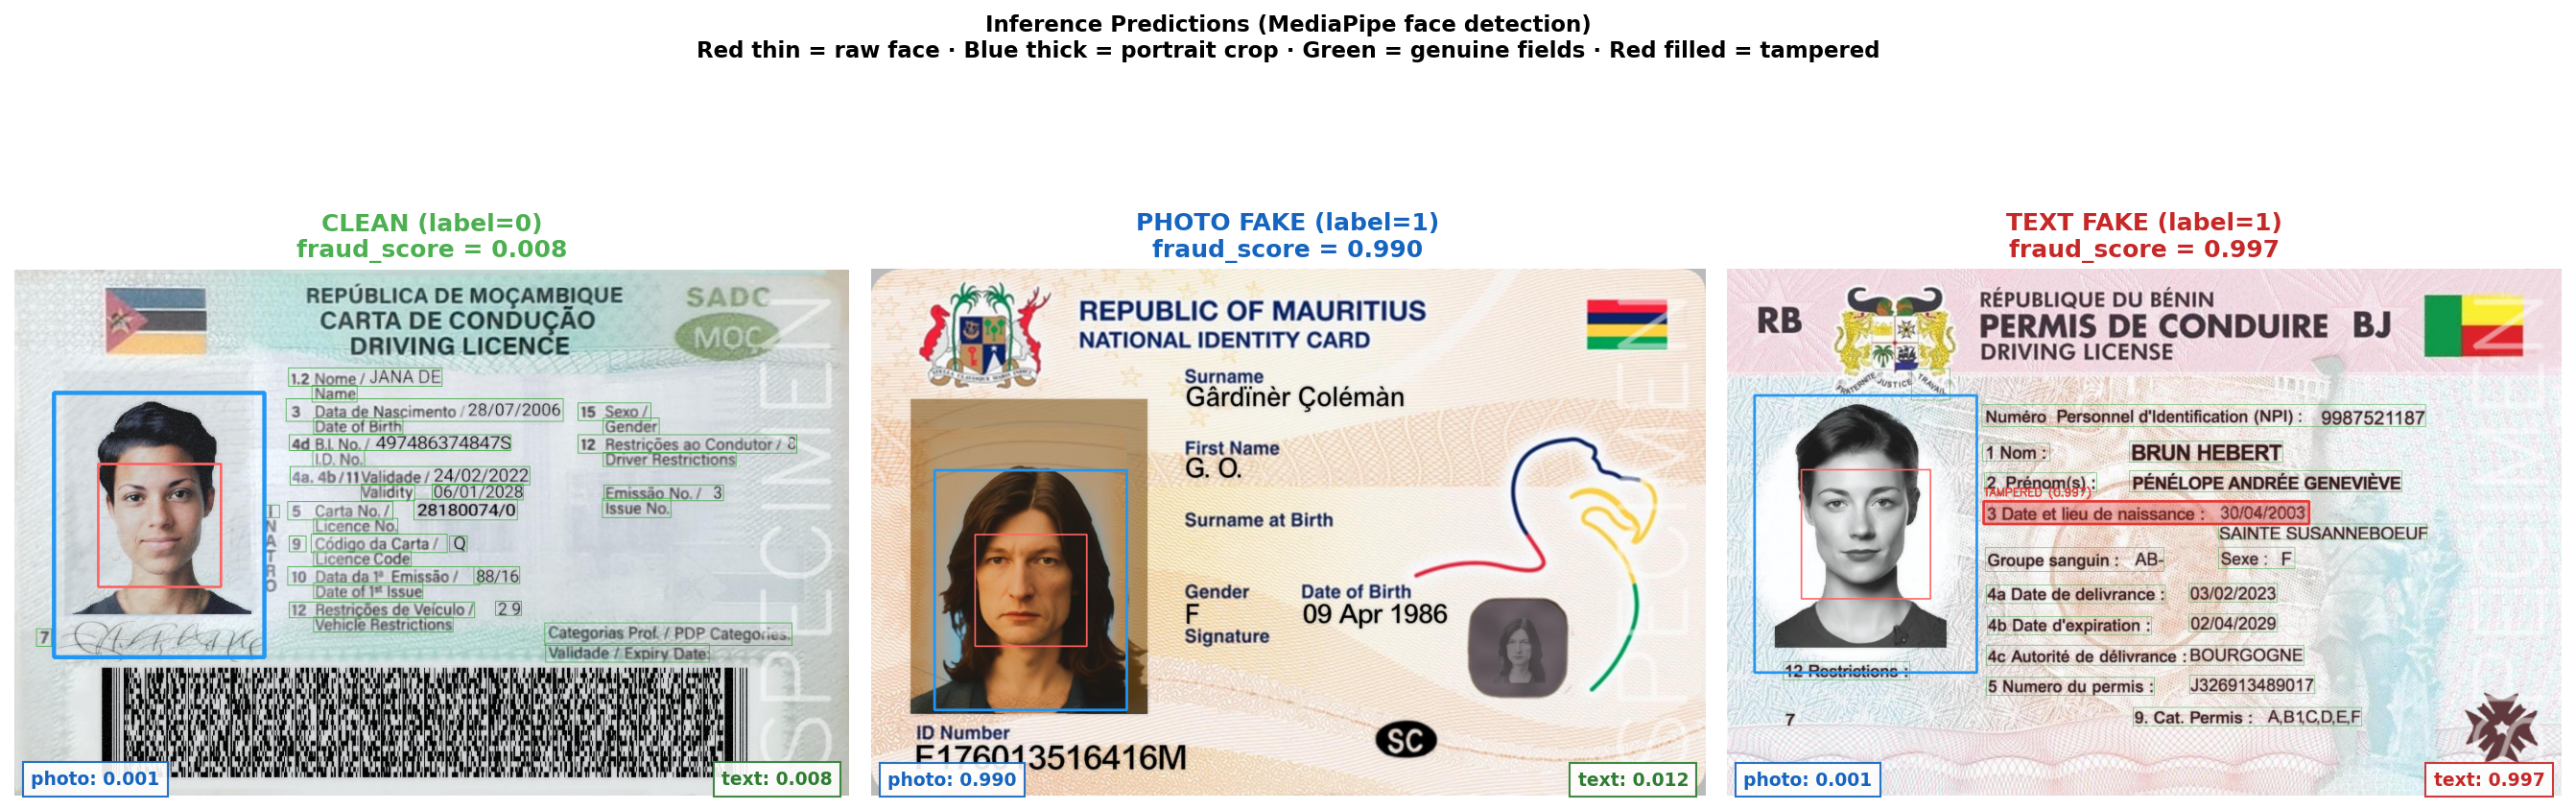
\includegraphics[width=\textwidth]{figures/inference_examples.png}
  \caption{Inference predictions on sample documents showing face detection
           (blue box), field scores (green=genuine, red=tampered), and
           final fraud score.}
  \label{fig:inference_examples}
\end{figure}

\subsection{Docker sandbox}

The Docker container is built from \texttt{nvidia/cuda:12.8.0-runtime-ubuntu22.04}
with Python~3.12 managed by \texttt{uv}.
All model weights, PaddleOCR detection models, and HuggingFace model configs
are baked into the image (no runtime or build-time downloads from HuggingFace).
Inference runs with \texttt{TRANSFORMERS\_OFFLINE=1}.

\begin{verbatim}
docker build -t freuid-repro .
docker run --rm --gpus all --network none \
  -v /path/to/images:/data:ro \
  -v $(pwd)/out:/submissions \
  freuid-repro:latest
\end{verbatim}

\subsection{Hardware and timing}

\begin{table}[H]
  \centering
  \small
  \caption{Inference timing for 142{,}818 documents.}
  \label{tab:timing}
  \begin{tabular}{lrr}
    \toprule
    Step & A100 GPU & Apple M3~Max \\
    \midrule
    MediaPipe face detection (CPU)     & 0.08\,h & 0.02\,h \\
    DINOv2-small face classification   & 0.05\,h & 0.03\,h \\
    PaddleOCR text field detection     & 1.4\,h  & 2.6\,h (CPU, 4 workers) \\
    ConvNeXt-B forensic panel scoring  & 1.2\,h  & 1.5\,h \\
    \midrule
    \textbf{Total}                     & \textbf{$\sim$2.7\,h} & \textbf{$\sim$4.1\,h} \\
    \bottomrule
  \end{tabular}
\end{table}

% ============================================================================
\section{Results}
\label{sec:results}

\begin{table}[H]
  \centering
  \caption{Main results. FREUID score is the official competition metric
           (lower is better).}
  \label{tab:results_main}
  \begin{tabular}{lccc}
    \toprule
    Evaluation & FREUID $\downarrow$ & AUC & Notes \\
    \midrule
    \multicolumn{4}{l}{\textit{Text subtask (ConvNeXt-B, max aggregation)}} \\
    \quad Train validation (1{,}807 docs) & 0.151 & 0.976 & Epoch 2/6 \\
    \midrule
    \multicolumn{4}{l}{\textit{Photo subtask (DINOv2-small)}} \\
    \quad Train validation (8{,}176 crops) & 0.005 & 0.998 & Epoch 6/8 \\
    \midrule
    \multicolumn{4}{l}{\textit{Combined (max of photo and text)}} \\
    \quad Public leaderboard & \textbf{0.294} & --- & Selected final submission \\
    \quad Private leaderboard & --- & --- & At submission time \\
    \bottomrule
  \end{tabular}
\end{table}

\subsection{Training progression}

\begin{table}[H]
  \centering
  \small
  \caption{ConvNeXt-B text model training progression (validation on 1{,}807
           held-out training documents, max aggregation).}
  \label{tab:training_epochs}
  \begin{tabular}{ccccrrc}
    \toprule
    Epoch & Loss & Panel AUC & Doc AUC & FREUID $\downarrow$ & APCER@1\% & TP/FP/FN \\
    \midrule
    1 & 0.427 & 0.954 & 0.973 & 0.155 & 25.3\% & 1306/154/8 \\
    \textbf{2} & \textbf{0.363} & \textbf{0.965} & \textbf{0.976} & \textbf{0.151} & \textbf{24.8\%} & \textbf{1309/118/5} \\
    3 & 0.330 & 0.968 & 0.974 & 0.165 & 26.9\% & 1312/98/2 \\
    4 & 0.298 & 0.977 & 0.926 & 0.330 & 47.5\% & 1313/219/1 \\
    5 & 0.279 & 0.979 & 0.967 & 0.206 & 32.7\% & 1312/110/2 \\
    6 & 0.267 & 0.978 & 0.970 & 0.238 & 37.3\% & 1311/105/3 \\
    \bottomrule
  \end{tabular}
\end{table}

Best model is at epoch~2: panel-level AUC continues improving after epoch~2, but
document-level FREUID worsens --- indicating overfitting to synthetic panel
distributions while losing generalization on real document scoring.

\begin{figure}[H]
  \centering
  % PLACEHOLDER: training curves
  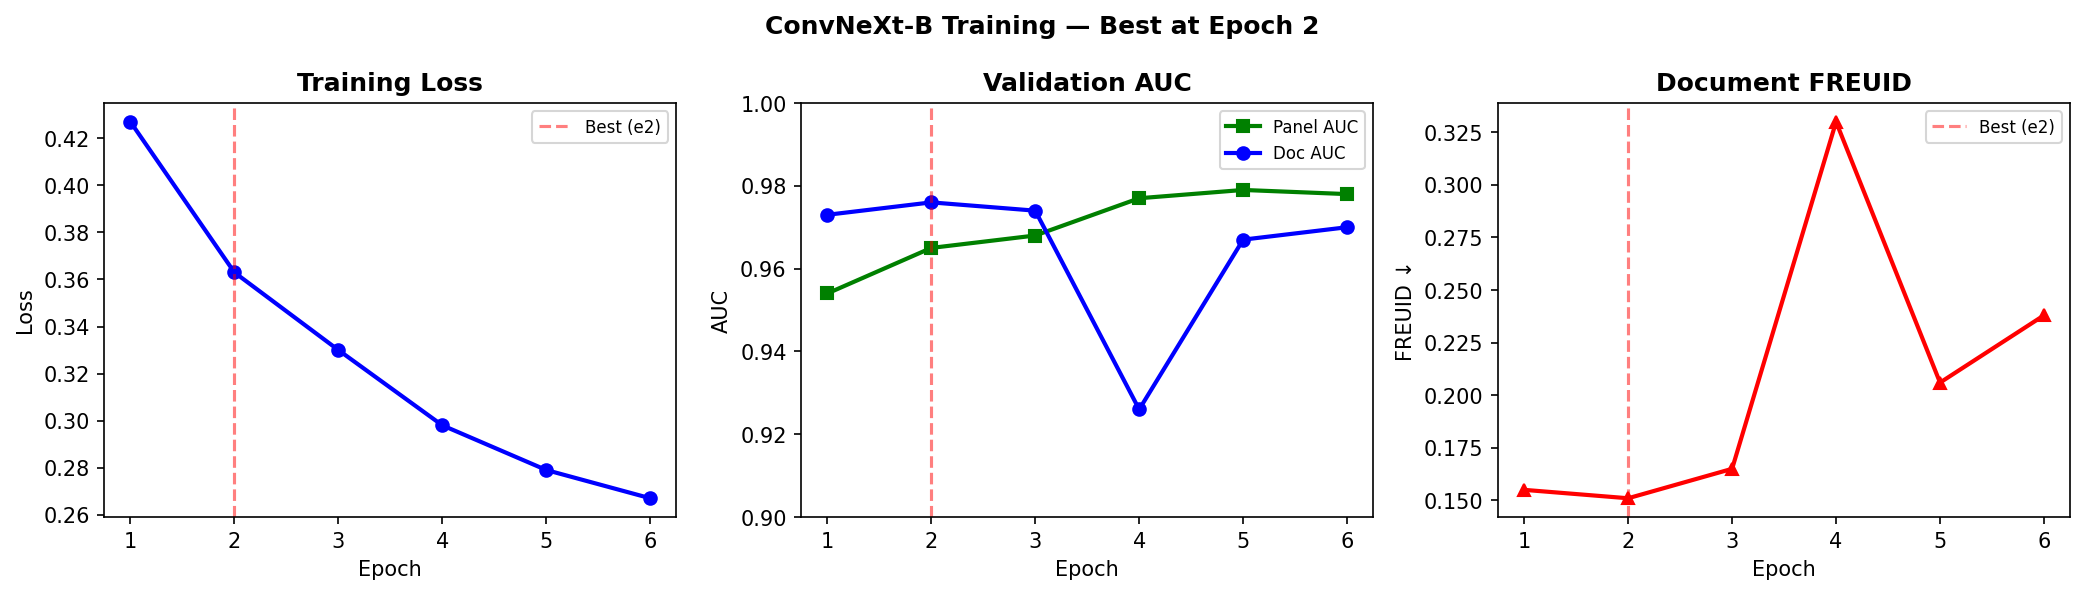
\includegraphics[width=0.9\textwidth]{figures/training_curves.png}
  \caption{Training progression showing panel AUC vs document FREUID divergence
           after epoch~2.}
  \label{fig:training_curves}
\end{figure}

% ============================================================================
\section{Reproducibility}
\label{sec:repro}

\begin{itemize}[noitemsep]
  \item \textbf{Repository:} \url{https://github.com/akhil838/doc-forensic-pipeline},
        commit \texttt{0d51c75d}.
  \item \textbf{Weights:} \url{https://huggingface.co/akhil838/doc-forensic-models-v1}
        (520\,MB total: ConvNeXt-B 336\,MB, DINOv2-small 85\,MB, BlazeFace 225\,KB,
        PaddleOCR 59\,MB).
  \item \textbf{Docker:} \texttt{docker build -t freuid-repro .}
        followed by \texttt{docker run --network none --gpus all}.
  \item \textbf{Dependencies:} Python 3.12, PyTorch 2.11+cu128, PaddlePaddle 3.3,
        transformers $\geq$5.10, timm 1.0.27. Full list in \texttt{requirements.txt}.
  \item \textbf{Training hardware:} Apple M3~Max (16-core CPU, 40-core GPU,
        64\,GB unified memory). Training time: $\sim$9 hours for text model
        (6 epochs), $\sim$1.3 hours for face model (8 epochs).
  \item \textbf{Inference hardware:} NVIDIA A100-PCIE-40GB.
        Wall-clock: $\sim$2.7 hours for 142{,}818 documents.
  \item \textbf{Randomness:} \texttt{SEED=42} for all random operations.
        Inference is deterministic given the same input order.
  \item \textbf{Network:} Inference runs with \texttt{--network none}
        (no runtime downloads). All weights baked into Docker image.
\end{itemize}

% ============================================================================
\section{Team and contributions}

Akhil Kosuri (sole participant): problem analysis, annotation tooling,
data pipeline, model architecture, training, inference engineering,
Docker packaging, and technical report.

\section*{Acknowledgments}

Thanks to the FREUID Challenge organizers (Microblink and IJCAI-ECAI 2026) for
providing the dataset and evaluation infrastructure.
Pre-trained models from Meta AI (DINOv2, DINOv3-ConvNeXt), Google (MediaPipe),
and PaddlePaddle (PaddleOCR) were instrumental to this solution.

\bibliographystyle{plain}
\bibliography{references}

% ============================================================================
\appendix
\section{Hyperparameters}
\label{app:hparams}

\begin{table}[H]
  \centering
  \small
  \caption{Complete hyperparameter listing.}
  \begin{tabular}{ll}
    \toprule
    \multicolumn{2}{l}{\textbf{Text tamper model (ConvNeXt-B)}} \\
    \midrule
    Backbone          & facebook/dinov3-convnext-base-pretrain-lvd1689m \\
    Unfrozen stages   & Last 2 (of 4) \\
    Panel size        & $224 \times 1008$ (6 tiles of $112 \times 336$) \\
    Hidden dim        & 1024 \\
    Head              & Linear(1024,256) $\rightarrow$ GELU $\rightarrow$ Drop(0.15) $\rightarrow$ Linear(256,1) \\
    Batch size        & 12 \\
    Learning rate     & $2 \times 10^{-5}$ \\
    Weight decay      & 0.01 \\
    Epochs            & 6 (best at epoch 2) \\
    Loss              & BCEWithLogitsLoss, pos\_weight=1.5 \\
    Scheduler         & Cosine annealing \\
    Gradient clipping & Max norm 1.0 \\
    Aggregation       & max \\
    Seed              & 42 \\
    \midrule
    \multicolumn{2}{l}{\textbf{Face model (DINOv2-small)}} \\
    \midrule
    Backbone          & facebook/dinov2-small \\
    Parameters        & 22M (all trainable) \\
    Input size        & $224 \times 224$ \\
    Portrait crop     & $256 \times 320$ (standardized) \\
    Head              & LayerNorm(384) $\rightarrow$ Drop(0.1) $\rightarrow$ Linear(384,2) \\
    Batch size        & 16 \\
    Backbone LR       & $10^{-5}$ \\
    Head LR           & $3 \times 10^{-4}$ \\
    Weight decay      & $10^{-4}$ \\
    Epochs            & 8 \\
    Loss              & CrossEntropyLoss \\
    Balanced samples  & 20{,}440 per class \\
    \midrule
    \multicolumn{2}{l}{\textbf{Field filtering}} \\
    \midrule
    TOP\_OCR\_IGNORE  & 0.17 (skip top 17\%) \\
    MIN\_W, MIN\_H    & 10, 8 pixels \\
    min\_aspect       & 0.5 (skip vertical) \\
    max\_h\_frac      & 0.09 (skip tall) \\
    max\_w\_frac      & 0.85 (skip wide) \\
    PAD\_X, PAD\_Y    & 15, 5 pixels \\
    MAX\_FIELDS       & 40 \\
    \bottomrule
  \end{tabular}
\end{table}

\section{Per-field prediction examples}
\label{app:field_predictions}

\begin{figure}[H]
  \centering
  % PLACEHOLDER: per-field prediction heatmap on a document
  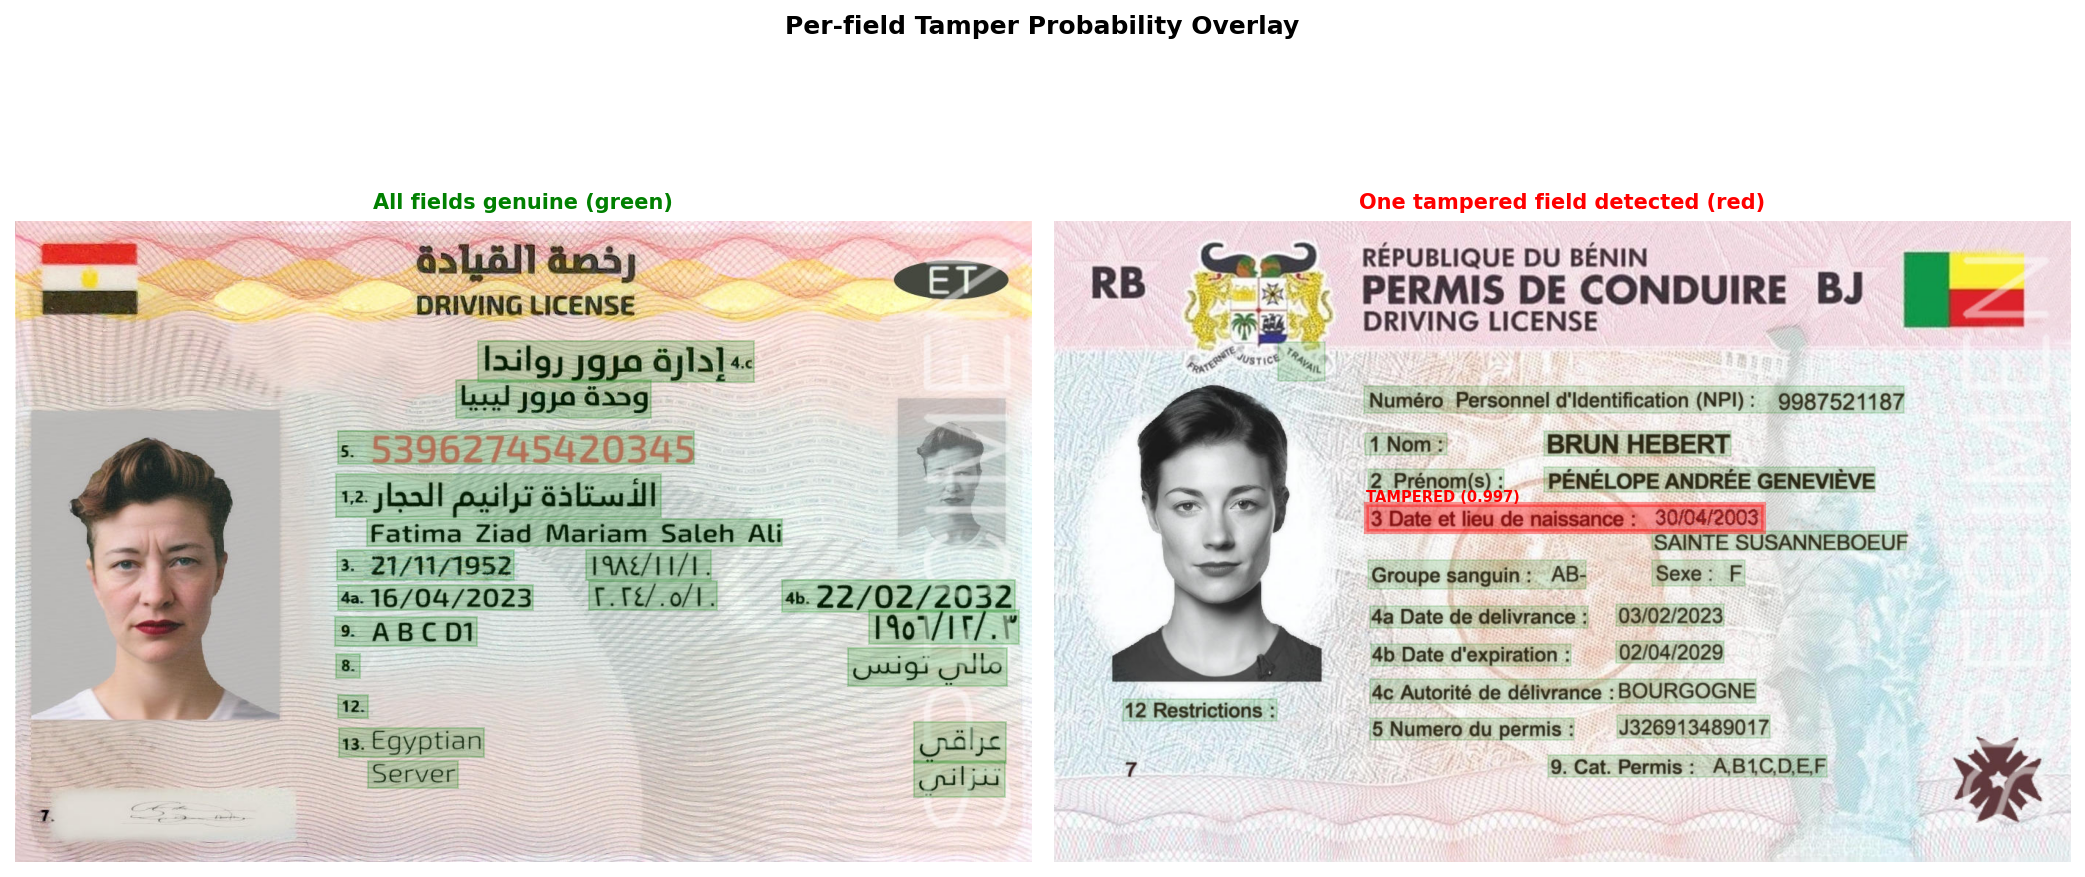
\includegraphics[width=\textwidth]{figures/field_heatmap.png}
  \caption{Per-field tamper probability overlay. Left: genuine document
           (all fields score $<0.1$). Right: tampered document (one field
           scores $>0.95$, others $<0.1$).}
  \label{fig:field_heatmap}
\end{figure}

\end{document}
